%%%%%%%% GRCON 2017 RABBIT EARS LATEX SUBMISSION FILE %%%%%%%%%%%%%%%%%

\documentclass{article}

\usepackage{times}
\usepackage{graphicx} % more modern
\usepackage{subfigure} 
\usepackage{natbib}
\usepackage{hyperref}
\usepackage{hyperref}
\usepackage{mathtools}
\def\navy
\usepackage{amsmath}

% please use this for your draft submission
\usepackage[nohyperref]{grcon2016} 
% please use this for your camera ready paper
%\usepackage[accepted]{grcon2016}

\grcontitlerunning{RFNoC \& Vivado HLS Challenge - Team Rabbit Ears: ATSC Receiver}

\begin{document} 

\twocolumn[
\grcontitle{RFNoC \& Vivado HLS Challenge \\
           Team Rabbit Ears: ATSC Receiver}

\ifdefined\navy
	\grconauthor{Andrew Valenzuela Lanez}{andrew.lanez@navy.mil}
\grconaddress{United States Navy}
\else
	\grconauthor{Andrew Valenzuela Lanez}{andrew.lanez@navy.mil}
\grconaddress{Space and Naval Warfare Systems Center Pacific (SSC Pacific), 53560 Hull St, San Diego, CA 92152 USA}
\fi
\grconauthor{Sachin Bharadwaj Sundramurthy, Alireza Khodamoradi}{\{sabharad, alirezak\}@eng.ucsd.edu}
\grconaddress{Department of Computer Science and Engineering, University of California, San Diego, La Jolla, CA 92093 USA}

\grconkeywords{software radio, gnu radio, dsp, GRCON, rfnoc, vivado hls, atsc receiver, dtv, digital television, rtl}
]

\vskip 0.3in

\begin{abstract} 
Creation of custom RFNoC (RF Network-on-chip) blocks that process a received ATSC (Advanced Television Systems Committee) signal is presented. The development workflow of RFNoC blocks may be perceived as complex and intimidating to some. Management of that workflow starting from Vivado HLS (High-Level Synthesis) 2015.4 and proceeding through the RFNoC framework is clarified with procedural steps. Coding and high-level synthesis optimization techniques that were used are discussed.
\end{abstract} 

\section{Introduction} \label{introduction}
The original digital television ATSC library was a contributing factor in the legal founding of GNU Radio. As interesting as it would be to delve into that historic moment, this paper instead details the effort put forth to evolve the venerable ATSC library as GNU Radio evolves with RFNoC. Real time playback of a live ATSC signal processed through the {\tt gr-dtv} ATSC receiver is possible on high-performance computers but not on most commodity computers \cite{corgan14}. This makes ATSC receiver blocks ideal candidates for porting into RFNoC. Computation intensive tasks can be offloaded to FPGA (field-programmable gate array) logic while applying high-level synthesis optimization techniques to improve receiver throughput. This can bring GNU Radio ever closer to achieving real time ATSC playback on a typical commodity computer.


\section{Contribution} \label{contribution}

RFNoC block contributions that have been verified to run on FPGA hardware are as follows: 

\begin{itemize}
\item \textbf{RFNoC: ATSC RX Filter}
	\begin{itemize}
	\item Vivado HLS Source \& Testbench
	\item NoC Block \& HDL Testbench
	\item UHD Integration \& GRC Bindings
	\item Settings Register Bus (partial 	integration)
	\end{itemize}

\item \textbf{RFNoC: ATSC Receiver FPLL}
	\begin{itemize}
	\item Vivado HLS Source \& Testbench
	\item NoC Block \& HDL Testbench
	\item UHD Integration \& GRC Bindings
	\item Settings Register Bus (partial 	integration)
	\end{itemize}

\item \textbf{RFNoC: DC Blocker}
	\begin{itemize}
	\item Vivado HLS Source \& Testbench
	\item NoC Block \& HDL Testbench
	\item UHD Integration \& GRC Bindings
	\item Settings Register Bus (partial 	integration)
	\end{itemize}

\item \textbf{RFNoC: AGC}
	\begin{itemize}
	\item Vivado HLS Source \& Testbench
	\item NoC Block \& HDL Testbench
	\item UHD Integration \& GRC Bindings
	\item Settings Register Bus (partial 	integration)
	\end{itemize}

\item \textbf{RFNoC: ATSC Viterbi Decoder}
	\begin{itemize}
	\item Vivado HLS Source \& Testbench
	\item NoC Block \& HDL Testbench
	\item UHD Integration \& GRC Bindings
	\end{itemize}

\item \textbf{RFNoC: ATSC Deinterleaver}
	\begin{itemize}
	\item Vivado HLS Source \& Testbench
	\item NoC Block \& HDL Testbench
	\item UHD Integration \& GRC Bindings
	\end{itemize}

\begin{itemize}
\item \textbf{RFNoC: ATSC Reed-Solomon Decoder}
	\begin{itemize}
	\item Vivado HLS Source \& Testbench
	\item NoC Block \& HDL Testbench
	\item UHD Integration \& GRC Bindings
	\end{itemize}
\end{itemize}

\item \textbf{RFNoC: ATSC Depad}
	\begin{itemize}
	\item Vivado HLS Source \& Testbench
	\item NoC Block \& HDL Testbench
	\item UHD Integration \& GRC Bindings
	\end{itemize}

\item \textbf{RFNoC: ATSC RX Filter-FPLL}
	\begin{itemize}
	\item Vivado HLS Source \& Testbench
	\item NoC Block \& HDL Testbench
	\item UHD Integration \& GRC Bindings
	\end{itemize}

\item \textbf{RFNoC: DC Blocker-AGC}
	\begin{itemize}
	\item Vivado HLS Source \& Testbench
	\item NoC Block \& HDL Testbench
	\item UHD Integration \& GRC Bindings
	\end{itemize}
\end{itemize}

Source code repository:
\begin{center}
\url{github.com/Xilinx/RFNoC-HLS-ATSC-RX}
\end{center}

\section{Design} \label{design}
The aforementioned blocks are functional counterparts of existing blocks in the {\tt gr-dtv} library. The rationale for porting those blocks is explained in the following.

\begin{figure}[h]
  \begin{center}
    \centerline{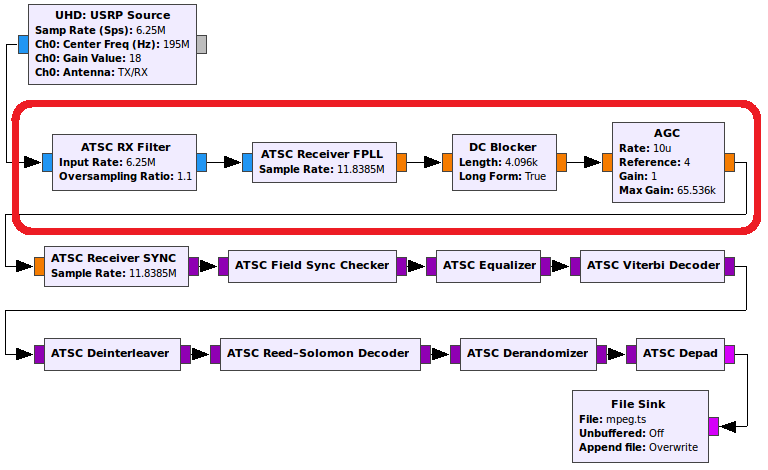
\includegraphics[width=\columnwidth]{gr_frontend.png}}
    \caption{Example flowgraph of ATSC receiver blocks from {\tt gr-dtv}. The four frontend blocks were among those chosen to port into RFNoC.}
    \label{uhd_atsc_rx}
  \end{center}
\end{figure}

The Ettus Research USRP X310 packaged with a Xilinx Kintex-7 XC7K410T FPGA was used for this design. RFNoC allows for up to ten user-specified CEs (computation engines or RFNoC blocks) to be programmed onto the XC7K410T. The decision on which blocks to port onto the FPGA hinged on two factors:

\begin{itemize}
\item[]  
{\em Frontend proximity.} Porting frontend blocks from software into hardware increases deterministic processing before the datastream falls under the whim of an operating system scheduler. RX Filter, FPLL, DC Blocker, and AGC were selected as shown in Figure~\ref{uhd_atsc_rx}.

\item[] 
{\em Bottlenecks.} Blocks that have higher consumption of runtime resources or cause buffers to fill are ideal candidates for porting. Figure~\ref{grruntime} shows the top runtime consumer is from Viterbi Decoder and secondary consumer is from Reed-Solomon Decoder so those blocks were targeted. The top buffer consumer in Figure~\ref{grbuffers} is from RX Filter.
\end{itemize}

Deinterleaver, Derandomizer, and Depad were eventually targeted due to their simplicity or for the sake of completeness around the FEC (forward error correction) blocks. Factoring in implementation challenges and deadlines, the blocks outlined in section \ref{contribution} were ultimately chosen.

\begin{figure}[h]
  \begin{center}
    \centerline{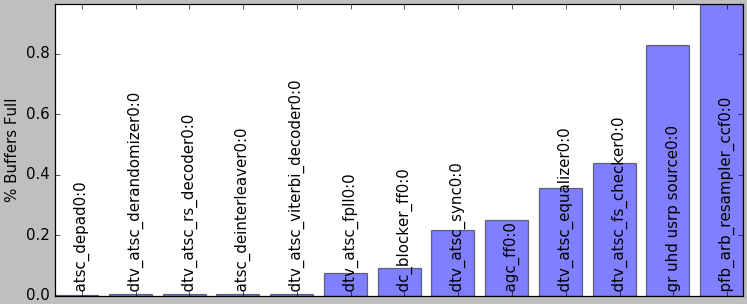
\includegraphics[width=\columnwidth]{gr_buffers.png}}
    \caption{Average buffer usage of {\tt gr-dtv} ATSC receiver blocks captured by ControlPort Performance Monitor.}
    \label{grbuffers}
  \end{center}
\end{figure}

\begin{figure}[h]
  \begin{center}
    \centerline{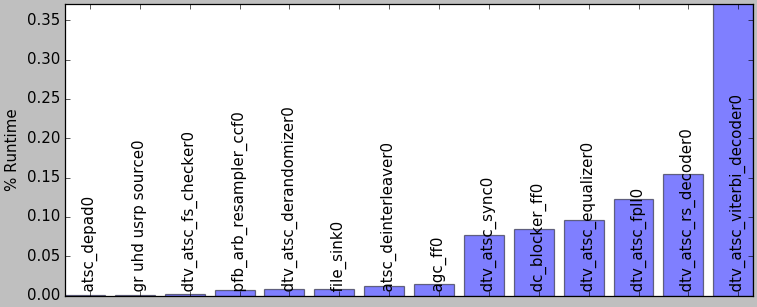
\includegraphics[width=\columnwidth]{gr_runtime.png}}
    \caption{Average runtime usage of {\tt gr-dtv} ATSC receiver blocks captured by ControlPort Performance Monitor.}
    \label{grruntime}
  \end{center}
\end{figure}

\begin{figure}[h]
  \begin{center}
    \centerline{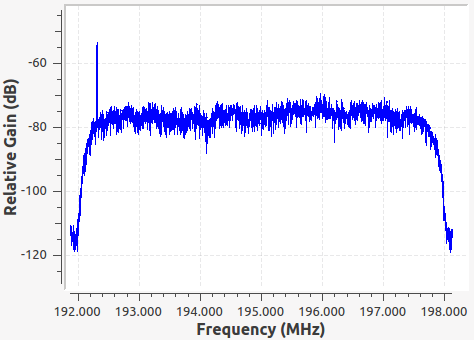
\includegraphics[width=\columnwidth]{spectrum.png}}
    \caption{Spectrum of live ATSC broadcast signal received by a 1byone (Figure~\ref{antenna}) antenna and USRP X310. Captured at the frontend between the DDC and RX Filter. 8VSB (Vestigal Side Band) modulation with 6 MHz bandwidth and pilot tone approximately 310 Khz above lower edge.}
    \label{spectrum}
  \end{center}
\end{figure}

Two key parameters in this receiver that drive sample rate requirements for all blocks are the 6.25 MHz sample rate coming out of the DDC (digital down coverter) at the receiver frontend and the oversampling ratio of the first block, RX Filter. It was decided that the 6.25 MHz input rate should not be modified to pass in a 6 MHz bandwidth (Figure~\ref{spectrum}) ATSC channel. Reasonable oversampling ratio values were found to range between 1.1 to 2 for the ATSC receiver software implementation to accumulate enough data to output video for playback. For an initial pass at implementing on hardware, it was decided to define target sampling rates based on the oversampling ratio of 1.1 to make implementation less constrained. Then, time permitting, iterate from there by increasing target rates and fine tune sample rates to match between blocks.

\section{Implementation} \label{implementation}
For each block, workflow started in Vivado HLS 2015.4 then proceeded into RFNoC. When ready, blocks were built into an FPGA image by running the {\tt make X310\_RFNOC\_HLS\_HG} command which called upon Vivado to synthesize the C++ code into a Verilog package and build a bitstream file. The bitstream file would then be programmed to the FPGA using {\tt uhd\_image\_loader}. Finally, a development iteration ended with testing in GNU Radio.

\begin{figure}[h]
  \begin{center}
    \centerline{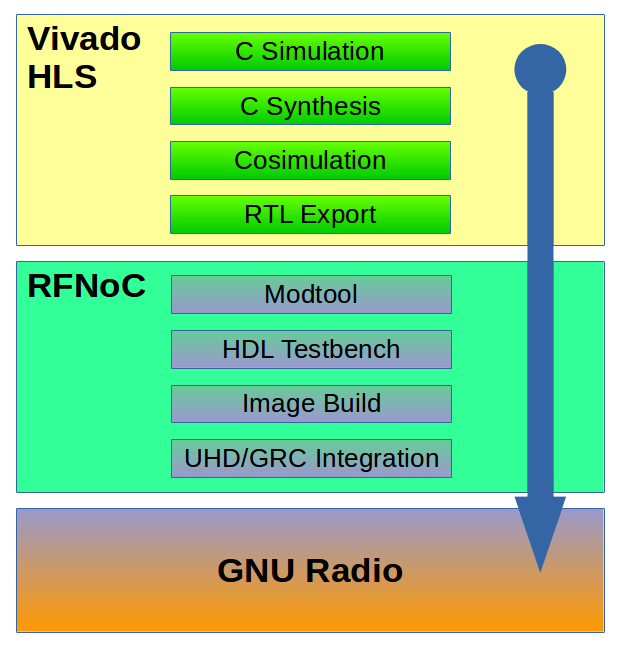
\includegraphics[width=\columnwidth]{workflow.png}}
    \caption{High-level progression of workflow.}
    \label{workflow}
  \end{center}
\end{figure}

Workflow in the RFNoC framework is already well documented at \cite{rfnockb}. The following discussion focuses on design implementation using Vivado HLS 2015.4 proceeded by challenges faced during implementation.

\subsection{Workflow in Vivado HLS}

\subsubsection*{Developing HLS Source}
Signal processing source files were written in C++ to be synthesizable. Vivado HLS optimization directives such as {\tt \#pragma HLS PIPELINE}, {\tt \#pragma HLS UNROLL}, {\tt \#pragma HLS RESOURCE}, and {\tt \#pragma HLS ARRAY\_PARTITION} were used. The tradeoff between optimizing to increase throughput versus optimizing to reduce utilization were kept in consideration. Detailed guidance on optimization techniques can be found at \cite{ug902}. Synthesizability could be checked using {\tt csynth\_design} (C Synthesis in Vivado HLS).

\subsubsection*{Developing HLS Testbench} A testbench was written in C++ to send input data to the DUT and compare the output against a golden output using {\tt csim} (C Simulation in Vivado HLS) in the C++ domain. The golden output was captured as a binary file using File Sink on the output of the counterpart or reference block in GNU Radio. Input was captured in a similar fashion with the original input source being a live ATSC signal fed from UHD: USRP Source. In the testbench, multiple function calls to the DUT per test run is encouraged to check the boundaries between returned output data sets and accumulate initiation interval statistics.

If {\tt csim} showed passing results and {\tt csynth\_design} showed the block to be synthesizable, then {\tt cosim} (C/RTL Cosimulation in Vivado HLS) was run to translate the C++ code into RTL (Verilog, VHDL, and/or SystemC) and apply the testbench input stimuli and output checking in the RTL domain. To synthesize the input port of the RX Filter block, for example, into the AXI Stream interface used in RFNoC, the {\tt \#pragma HLS INTERFACE axis depth=64 port=in} was used on the top level function of the block. The {\tt depth} parameter has no bearing on synthesis. Instead, it is a control parameter for the {\tt cosim} testbench to know how to size its input FIFO so it matches the RX Filter input array size which does have bearing on synthesis.

Extra sanity checks were sometimes made after modifying the HLS testbench to dump DUT output values into a binary file. The binary output file was then used in a File Source block at the appropriate location in the GNU Radio ATSC receiver example. For example, if the binary file was generated from the RX Filter DUT and its HLS testbench, the UHD: USRP Source and RX Filter blocks in GNU Radio were replaced by a File Source block pointing to that binary file. This way, GNU Radio could perform more checks against the DUT output and report meaningful information such as sync errors. This also tested whether the quality of the binary data was sufficient for decoding into video. Effectively, a block completed this early on in HLS could momentarily bypass RFNoC for basic testing in GNU Radio.

\begin{figure}[h]
  \begin{center}
    \centerline{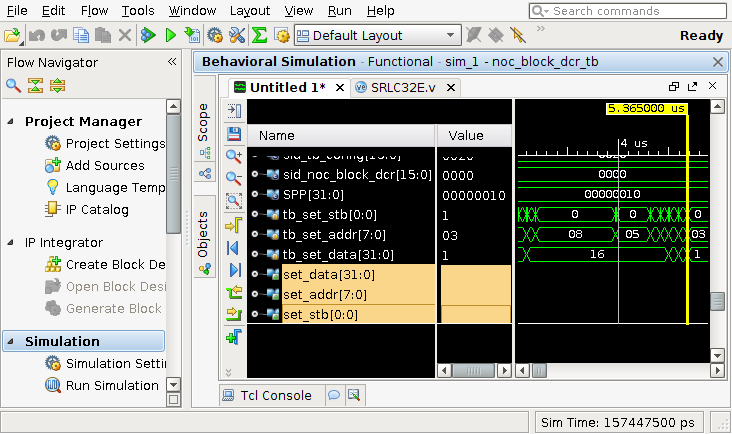
\includegraphics[width=\columnwidth]{xsim.png}}
    \caption{The HDL testbench uses Vivado Simulator or XSIM. The GUI as shown can be enabled using {\tt make noc\_block\_[BLOCK NAME]\_tb GUI=1}. The logic analyzer feature was used here to observe DC Blocker settings bus signals.}
    \label{xsim}
  \end{center}
\end{figure}

\subsubsection*{Iterating Between HLS and RFNoC}
After a block passed {\tt cosim}, it was ready to test against the RFNoC HDL testbench. {\tt export\_design} (Export RTL in Vivado HLS) was used to convert the C++ source files into Verilog and Xilinx XCI IP source files. Those files became the DUT in the RFNoC HDL testbench. The binary input and golden output files used in HLS were converted to ASCII representations using MATLAB (Python would have worked as well) which were then used as input and golden output array variables in the SystemVerilog HDL testbench. If the DUT had bugs revealed by the HDL testbench (Figure~\ref{xsim}) or by running its FPGA implementation in GNU Radio, it was debugged in HLS or HDL testbench, re-packaged with {\tt export\_design}, then retested. This process was repeated until the RFNoC block implementation functioned as desired in GNU Radio.

\subsection{Challenges} \label{challenges}
The scheduler is a noteworthy feature of GNU Radio dataflow that is not accessible to RFNoC blocks. The software implementation of RX Filter uses the {\tt set\_history()} function to recall samples from the previous set of inputs. If not for this feature, the polyphase FIR filterbank--theory from \cite{harris04}--in RX Filter would output starting transients whenever a new set of samples is filtered. {\tt set\_history()} prepends the incoming samples with trailing samples from the previous input. Filterbank phase arms are adjusted such that the starting transient overlaps in phase with the previous ending transient. The overlapping transients are then not sent to output (overlap-and-discard method). The RFNoC: ATSC RX Filter block cannot access {\tt set\_history()} so previous input samples (specifically the last 18) must be stored internally in FPGA logic then fed into the filterbank before the next set of input samples arrive. Considerations like this must be made when porting existing GNU Radio blocks into RFNoC.

An oddity was found while testing the RFNoC: ATSC Receiver FPLL block in GNU Radio. All samples were being output with a gain of $\mathtt{3.276700480546441\times10^{4}}$ applied over their expected values. This gain did not manifest when running the HLS testbench nor the HDL testbench.  To resolve this, the FPLL HLS source file was modified to simply divide all outputs by that gain. Of course, the HLS and HDL testbenches had to be updated to multiply that gain back onto the outputs before checking them. The source of this mysterious gain was never found.

The GNU Radio implementation of DC Blocker has a default setting of processing 4,096 samples in and out and using a "long form" of nested loops in its moving averager. Using these parameters in the initial HLS implementation, the DUT would pass {\tt csim} but {\tt cosim} would timeout after running for more than 24 hours. This may be due to the enormous estimated maximum initiation interval of 251,969,541 clock cycles reported by {\tt csynth\_design}. The target initiation interval $\mathtt{II}$ in clock cycles can be calculated as

\begin{equation}\label{ii}
\mathtt{II = \lfloor\frac{f_{CE\_CLK}}
{f_{s}}\times{n}\rfloor}
\end{equation}

where $\mathtt{f_{CE\_CLK}}$ is the computation engine clock rate, $\mathtt{f_{s}}$ is the sample rate, and $\mathtt{n}$ is the number of samples processed. Given the CE clock is $\mathtt{f_{CE\_CLK} = 214\ MHz}$, the required output sample rate determined from studying the receiver in Figure~\ref{uhd_atsc_rx} is $\mathtt{f_{s} = 11.8385\times10^{6}\ MS/s}$ (megasamples per second), and the number of output samples per function call to DC Blocker is $\mathtt{n = 4,096}$, applying these values to equation \ref{ii} the target initiation interval becomes $\mathtt{II = 2,314\ clock\ cycles}$. To minimize clocks, it was decided to reduce the delay line length and not use "long form" so that less nested loops were used with two delay lines instead of four in the moving averager. The DC Blocker software implementation could still synchronize with and decode a live ATSC signal with minumum delay line length 128 (which changed the $\mathtt{II}$ target to 2,315) and "long form" disabled. After applying these changes to the HLS source code, initiation interval reduced to 207,365 clock cycles. Optimization directives {\tt \#pragma  HLS ARRAY\_PARTITION} with {\tt cyclic factor=16} applied to both delay lines and {\tt \#pragma HLS UNROLL factor=16} applied to nested loops brought initiation interval down to 31,671 clock cycles. The optimizations were still not enough to meet the target initiation interval. Setting the unroll and cyclic factor parameters to 64 reduced initiation interval to 6,543 with no errors or warnings in HLS. However, image build resulted in a critical warning on timing and the RFNoC implementation functioned erratically in hardware. This was a recurring issue and further discussion on this is in Section \ref{results}.

The Viterbi block underwent a similarly radical improvement in optimization. An earlier implementation of the Viterbi algorithm relied on many loops and nested loops. It had a 2,659,376 clock cycle initiation interval though the target was 163,124 clock cycles. Vivado HLS was found to not be unrolling loops that greatly would benefit from being pipelined. Calls to the same function within the loops may have been a reason the loops could not be unrolled. These functions were copied many times and numbered to match loop iterations and loops were manually unrolled. This enabled more pipelining and reduced initiation interval to 138,920 which met the target.

\begin{figure}[h]
  \begin{center}
    \centerline{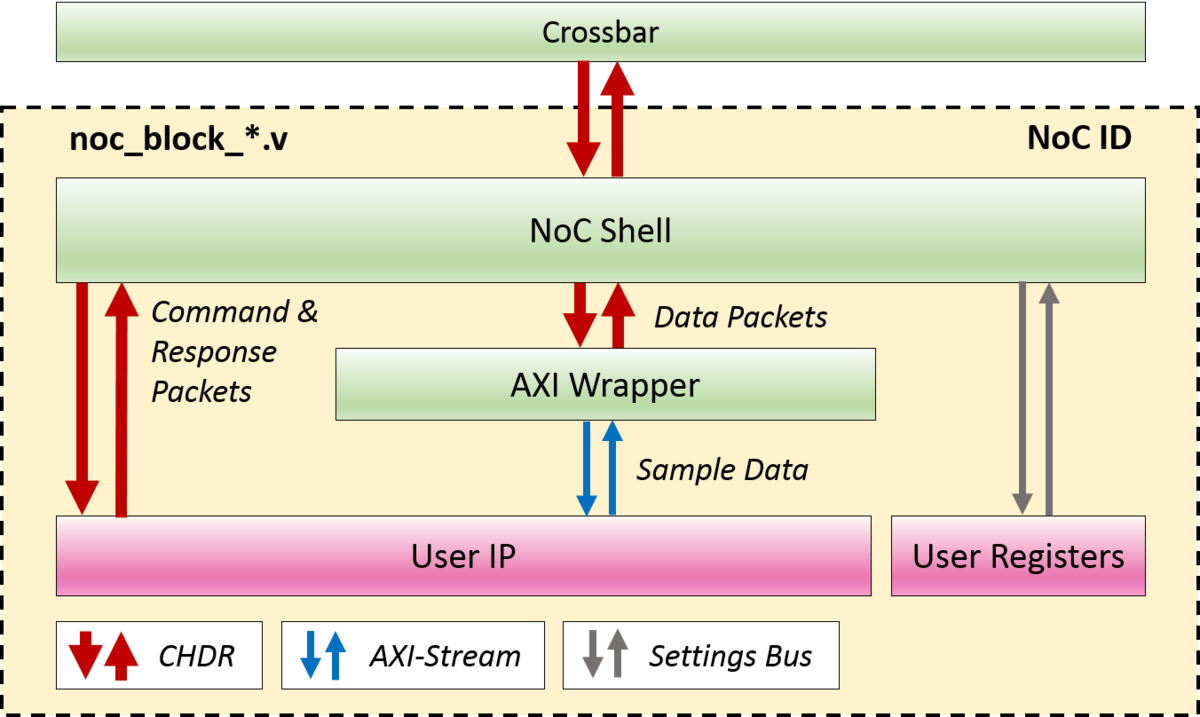
\includegraphics[width=\columnwidth]{noc.png}}
    \caption{CHDR (compressed header, an Ettus-specific protocol) packets pass between AXI Wrapper, NoC Shell, and Crossbar and between User IP and NoC Shell. Information and image retrieved from \cite{rfnockb}.}
    \label{noc}
  \end{center}
\end{figure}

Throttle and RFNoC: FIFO blocks were used  (Figure~\ref{grc}) to compensate for mismatching sample rates. As more RFNoC blocks were developed, more RFNoC: FIFO instances were needed, pushing total block count closer to the 10 CE limitation on the USRP X310. A solution was to combine blocks at the HLS level. RX Filter arbitrarily outputs either 60 or 61 pairs of float (IQ) samples at a time. FPLL requires one pair of float samples in to output a single float at a time. Hence, no dynamic FIFO was needed in between when combining the two into one RFNoC: ATSC RX Filter-FPLL block. DC Blocker, however, requires a rigid 128 samples in and out. AGC only requires one sample in and out so it was combined with DC Blocker at the HLS level to implement RFNoC: DC Blocker-AGC. Combining blocks at the HLS or User IP level to increase available CE slots came at the cost of a slight decrease in overall sample rate but overhead incurred from packetization (Figure~\ref{noc}) was eliminated.

\begin{figure}[h]
  \begin{center}
    \centerline{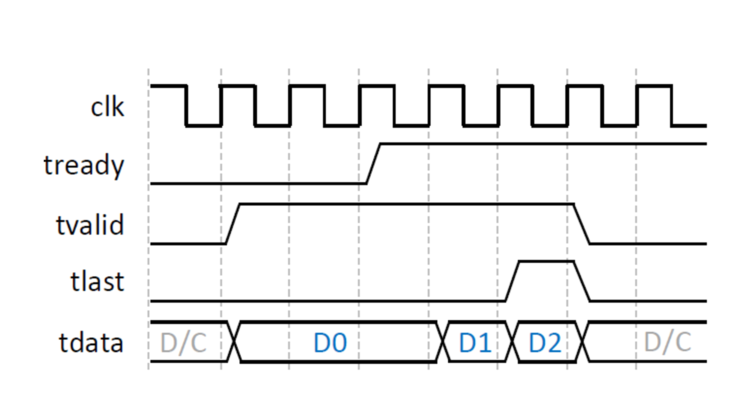
\includegraphics[width=\columnwidth]{axis.png}}
    \caption{AXI Stream signals. Image retrieved from \cite{rfnockb}.}
    \label{axis}
  \end{center}
\end{figure}

\begin{figure}[h]
  \begin{center}
    \centerline{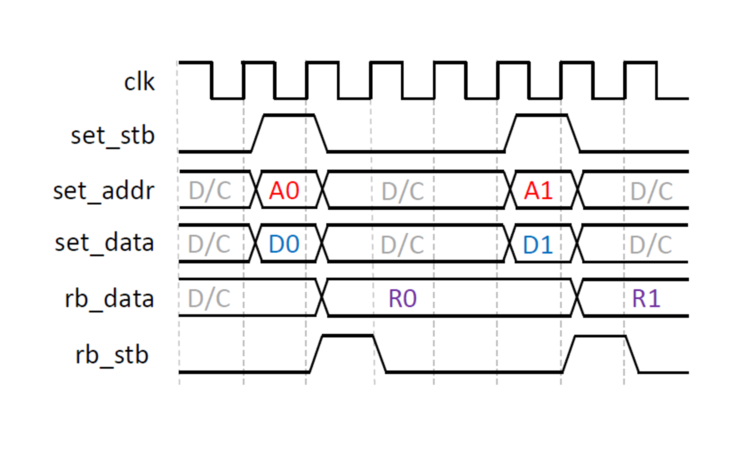
\includegraphics[width=\columnwidth]{settings.png}}
    \caption{Settings Bus signals. Image retrieved from \cite{rfnockb}.}
    \label{settings}
  \end{center}
\end{figure}

Provisions for the settings register bus were implemented in HLS source, HLS testbench, NoC block, HDL testbench, UHD integration, and GRC binding files. Values were not observed to be propagating to the settings registers in Vivado Simulator (Figure~\ref{xsim}). It was questionable whether the settings bus ports were getting synthesized correctly from HLS source files. Guidance for synthesizing AXI Stream interface ports is well documented in \cite{ug1037}. The {\tt \#pragma HLS INTERFACE axis} directive is used to synthesize ports that match the AXI stream signals used by RFNoC in Figure~\ref{axis}. Similar documentation for synthesizing the settings bus signals shown in Figure~\ref{settings} could not be found. The {\tt \#pragma HLS INTERFACE ap\_stable} and {\tt \#pragma HLS INTERFACE ap\_none} directives described in \cite{ug902} were experimented with to attempt synthesis of the {\tt set\_addr}, {\tt set\_data}, {\tt set\_stb} settings bus ports from HLS source files. They are data port interface directives, however, have no associated I/O protocol. Regardless, the settings registers were implemented on FPGA and tested in GNU Radio and did not function as desired. This is why settings bus is marked "with partial integration" in section \ref{contribution}.

\section{Results} \label{results}

This section presents the resulting BRAM (Block RAM), DSP, FF (flip-flop), and LUT (lookup table) utilization and sample rates of the RFNoC blocks. Live performance of the RFNoC blocks running in GNU Radio is then discussed.

\begin{figure}[h]
  \begin{center}
    \centerline{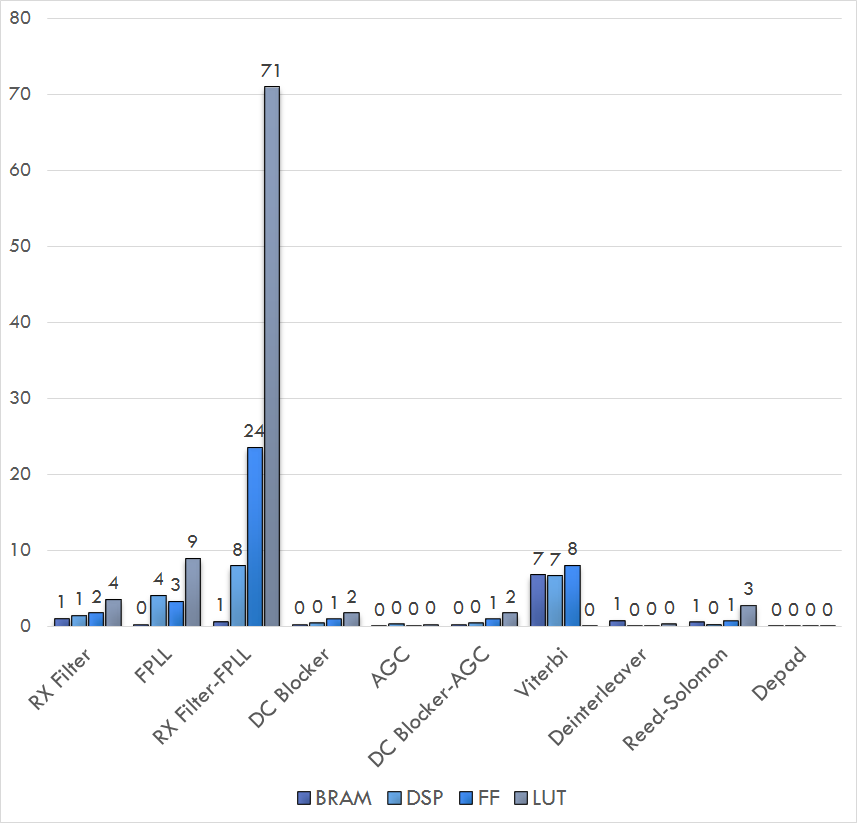
\includegraphics[width=\columnwidth]{percentarea.png}}
    \caption{RFNoC block percent utilization based on values from Table~\ref{area}.}
    \label{percentarea}
  \end{center}
\end{figure}

\begin{table}[h]
  \begin{center}
    \caption{RFNoC block utilization area reported by Vivado HLS C Synthesis in terms of units. These blocks were verified to function properly in hardware.\\
    }
    \centerline{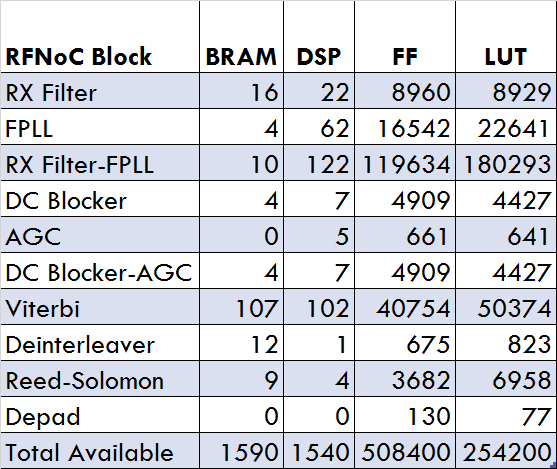
\includegraphics[width=\columnwidth]{area.png}}
    \label{area}
  \end{center}
\end{table}

It is worth noting the outlying 71\% LUT utilization of RX Filter in Figure~\ref{percentarea}. An alternate version was developed that uses 17\% but with about 44\% slower throughput. Higher utilization may be attributed to the use of more optimizations and hardcoding all polyphase and differential filterbank tap values rather than using loops to calculate a prototype filter and more loops to partition the prototype filter into a polyphase filter and calculate a differential filter. A consequence of hardcoding these tap values is the oversampling ratio parameter can no longer be adjusted. In the 17\% utilization version of RX Filter, adjusting oversampling ratio variable {\tt sps} from HLS source code initializes the calculation of all filter taps so that they support the oversampling ratio. Provisions to adjust that oversampling ratio from GNU Radio Companion was attempted with the partial integration of the settings bus.

\begin{table}[h]
  \begin{center}
    \caption{RFNoC block sample rates were calculated by applying initiation intervals reported by Vivado HLS Cosimulation and the 214 MHz CE clock value to equation \ref{ii} without the floor operator and solving for $\mathtt{f_{s}}$. Target output rates were calculated by multiplying the 6.25 MHz receiver input rate with a factor determined by the internal functionality of each respective block. RX Filter samples per output is an average of its arbitrarily resampled output and an irrational number. Blocks denoted with "v2" were optimized for higher throughput but function erratically on hardware.\\
    }
    \centerline{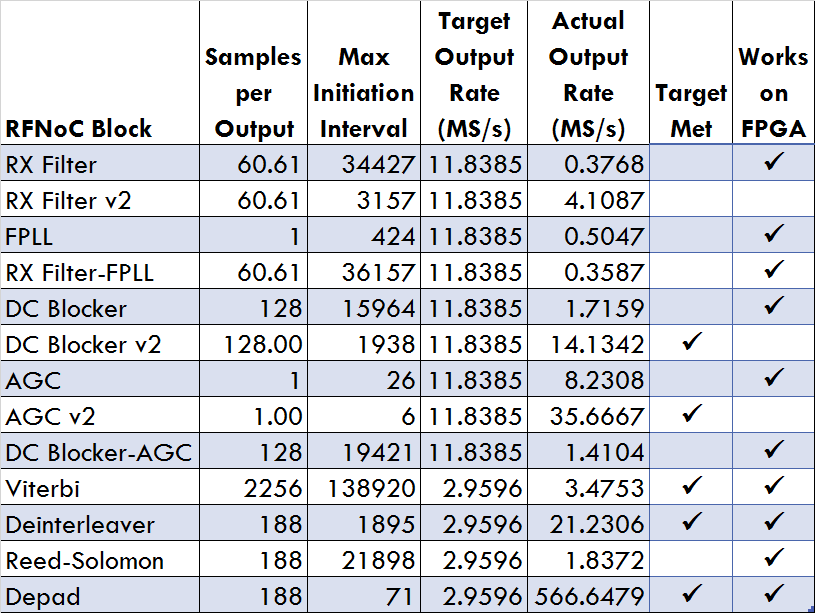
\includegraphics[width=\columnwidth]{rates.png}}
    \label{rates}
  \end{center}
\end{table}

In some instances, the RFNoC image build process resulted in a critical warning for timing not being met. This was despite Vivado HLS 2015.4 giving no indication of timing not being met from {\tt csynth\_design}, {\tt cosim}, nor {\tt export\_design} with the Evaluate Verilog option enabled. Examples of this are the "v2" labeled blocks in Table~\ref{rates}. They were significantly optimized to approach or exceed target throughputs. No issues were reported from Vivado HLS 2015.4, however, the image builder reported critical warnings on timing and those blocks functioned erratically on hardware (could not synchronize, junk data, etc.).  This was despite HDL testbench showing passing results. Sometimes painfully, one optimization had to be removed at a time between image builds to isolate the offending optimization responsible for the critical warning or erratic behavior. This put an invisible limit on allowable optimizations and made target sample rates in a working hardware implementation unreachable. However, before iterating back optimizations, it was always worth testing an image on hardware; on a few fortunate ocassions the image functioned as desired despite critical warnings.

\ifdefined\navy
\begin{figure}[h]
  \begin{center}
    \centerline{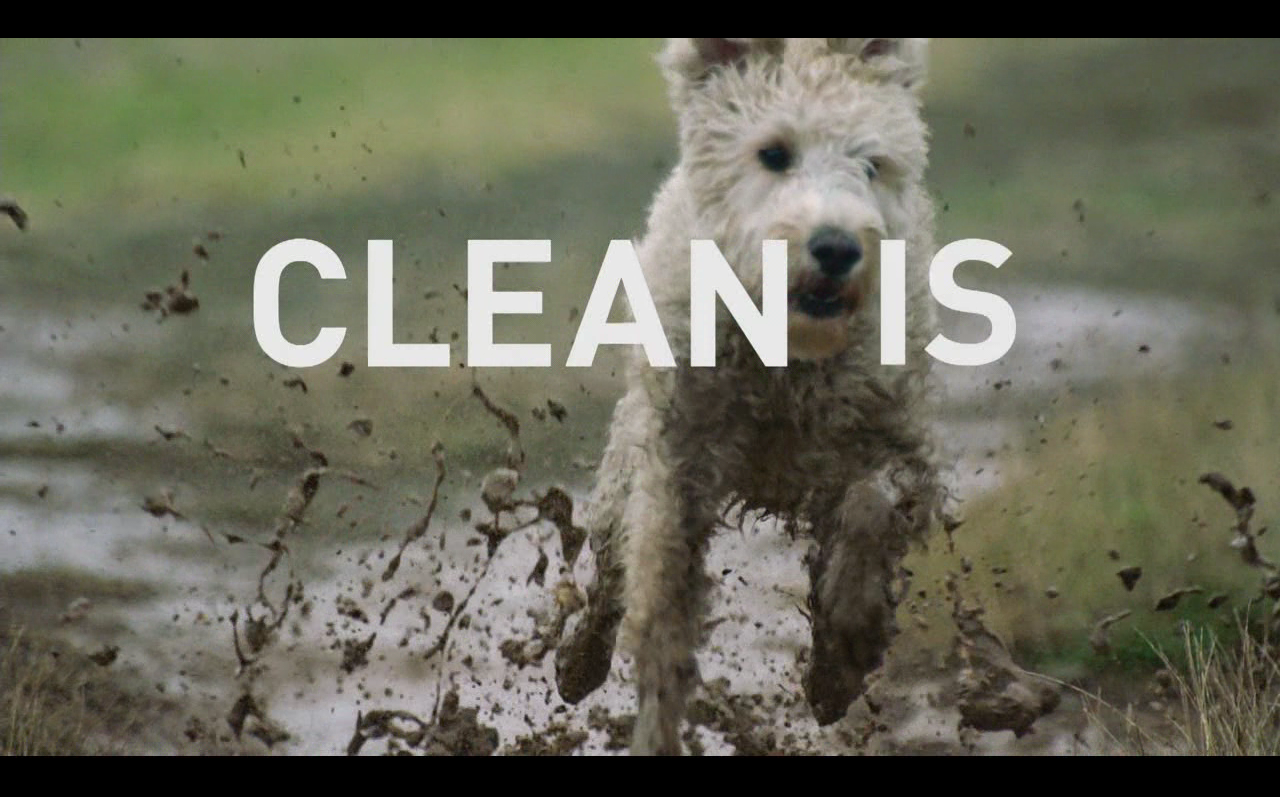
\includegraphics[width=\columnwidth]{dog.png}}
    \caption{Screenshot of video from a live ATSC signal that was processed through implemented RFNoC blocks.}
    \label{dog}
  \end{center}
\end{figure}
\fi

Synchronization and decoding into playable video (Figure~\ref{dog}) and audio was achieved but, because target sample rates were unmet (Table~\ref{rates}), video playback was not approaching real time as originally desired. Placing RFNoC: FIFO blocks in front of specific RFNoC blocks and a Throttle block after the DDC as shown in Figure~\ref{grc} allowed for processing of a live ATSC signal into playable video and audio but with five to ten times more latency than the pure software version of the receiver and with chunks of samples being dropped. A couple seconds of audio and video would render from a decoded output data size ranging anywhere between 20 to 50 megabytes.

\begin{figure}[h]
  \begin{center}
    \centerline{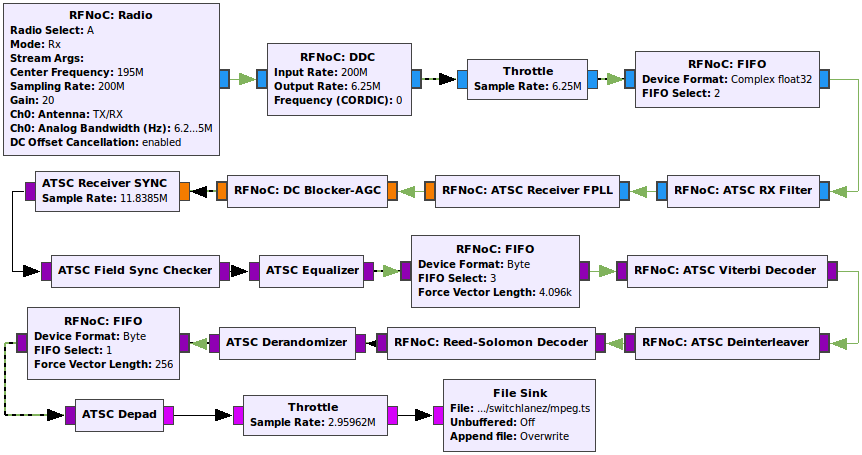
\includegraphics[width=\columnwidth]{grc.png}}
    \caption{Flowgraph with RFNoC blocks implemented and RFNoC: FIFO blocks placed to mitigate dropping of samples.}
    \label{grc}
  \end{center}
\end{figure}

For the sake of finding new avenues to improve sample rates, very brief experimentation was done with Vivado HLS 2017.1. Optimizations to RX Filter that failed to meet timing in version 2015.4 were passing in version 2017.1. A single afternoon of further optimizing RX Filter in version 2017.1 netted a ten-fold improvement in sample rate over the 2015.4 optimized version. That huge leap in improvement was accomplished in an extremely short time span relative to the month spent optimizing RX Filter in version 2015.4 to net only a 40\% improvement. Optimizing DC Blocker in Vivado HLS 2017.1 netted similar improvements. AGC was below its target sample rate in 2015.4 but exceeded its target by a factor of three in 2017.1. This all made Vivado HLS 2017.1 seem very promising. However, attempting to build an image with Vivado 2017.1 linked to RFNoC failed because RFNoC did not support the Xilinx IP generated by Vivado 2017.1 HLS. Regardless, this finding shows great promise if future revisions of RFNoC were to support newer and seemingly improved versions of Vivado HLS. It seems to be common opinion that coding in pure Verilog is the best way to meet timing and throughput requirements. That gap appears to be closing rapidly as improved versions of Vivado HLS are released.

\section{Lessons Learned} \label{lessonslearned}

A shotgun approach to this project was used by selecting many blocks to port into RFNoC with hopes of hitting the bullseye. With Viterbi being the largest resource consumer and bottleneck and its RFNoC implementation working and meeting the target throughput, it can be considered that a bullseye was hit. Multiple other blocks struck right around the mark. Simpler blocks such as Deinterleaver and Depad far surpassed target sample rates and only came about to be developed during times when little to no progress could be made on more challenging blocks such as RX Filter, DC Blocker, and Viterbi. This approach may have been inefficient at times with efforts being spread thin across many blocks. It is uncertain whether a more focused, sniper approach on fewer blocks would have yielded better results.

Image builds took two to three hours on higher performance workstations in the UCSD SeaLab. But with the majority of build attempts being done from home on an HP laptop, it took about seven hours per build. It wasn't until the final weeks of the project that a novice Linux user discovered the {\tt indicator-cpufreq} package for Ubuntu. Build times were then reduced to about five hours. It also helped to convert a Windows Surface Pro 3 tablet to dual boot with Ubuntu 16.04.1 so two images could be built simultaneously. Further, multiple instances of Vivado HLS 2015.4 could be running on both machines while both were also building images. Resourceful tricks to streamline productivity are fruitful for projects of this nature.

\begin{figure}[h]
  \begin{center}
	\ifdefined\navy
    	\centerline{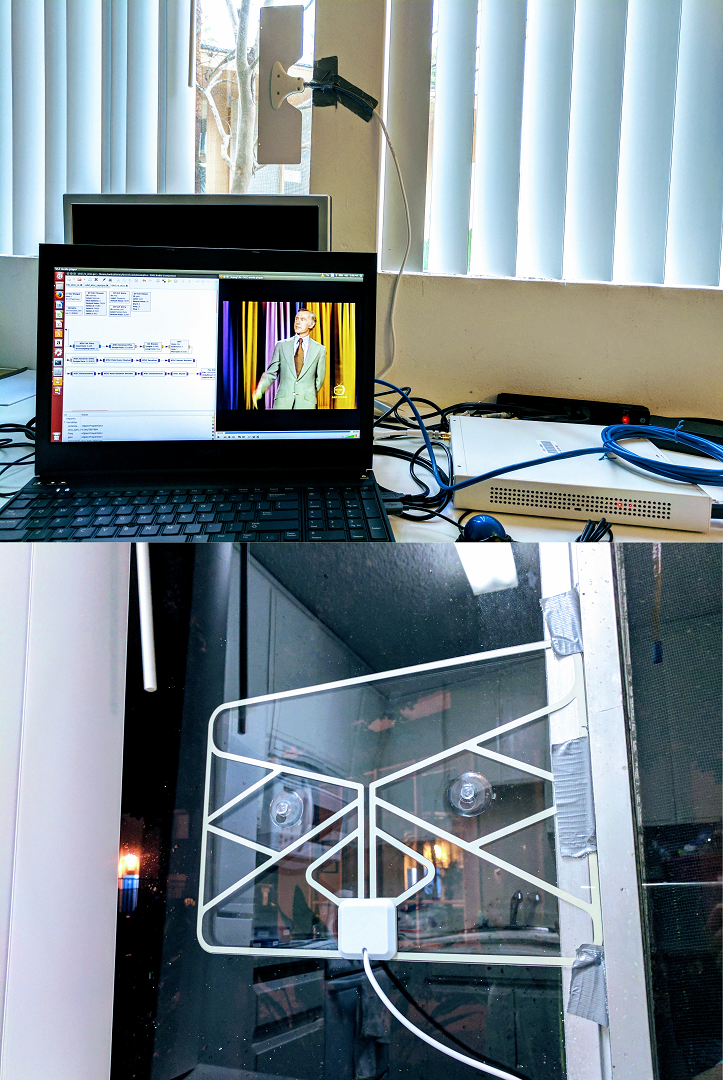
\includegraphics[width=\columnwidth]{antenna.png}}
	\else
    	\centerline{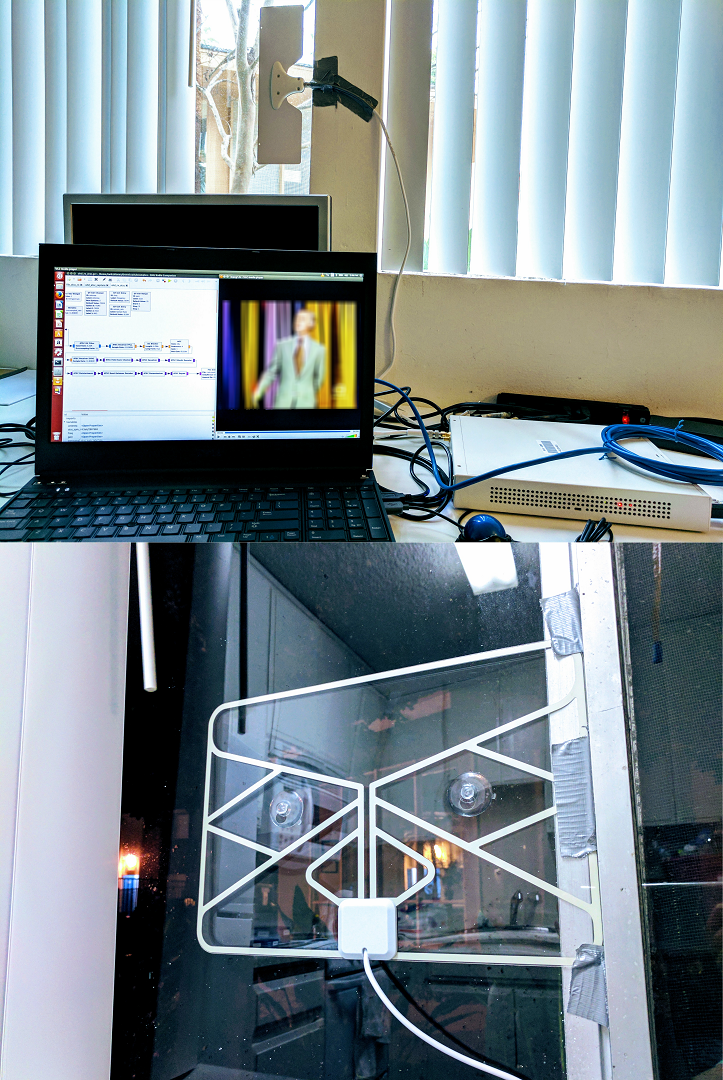
\includegraphics[width=\columnwidth]{antenna_blur.png}}
    \fi
    \caption{Top: Mohu Leaf antenna connected to a USRP X310. This antenna was eventually returned to the vendor due to poor reception. Bottom: 1byone antenna had consistent reception of the 195 MHz-centered ATSC channel at this specific position on the window and was used for primary testing.}
    \label{antenna}
  \end{center}
\end{figure}

Initial difficulties with getting any signal in the primary test location was resolved by changing from a 25-mile advertised range Mohu Leaf to a 50-mile advertised range 1byone antenna. The latter came bundled with an amplifier but performed better with the amplifier switched off. There was one specific position on the window (Figure \ref{antenna}) and one channel (ABC Network) at 195 MHz where the received signal (Figure~\ref{spectrum}) was acceptable. Testing had been done very early on in the project in a different location with a higher grade antenna resulting in higher reception quality signified by a smaller receiver output file playing back a longer duration of video. But access to that location was very limited and those tests had been done before any RFNoC blocks were developed. More testing in the better location with better antenna is a future action item.

It was realized partway through the project that real time playback was ambitious based on timing estimates reported by Vivado HLS. The ATSC standard \cite{atsc} states that an  MPEG-2 Transport Stream (MPEG-2-TS) is broadcast at a rate of 19.39 Mbps (megabits per second). The {\tt gr-dtv} ATSC receiver processed a live signal into a video file with a 15.128 kbps (kilobits per second) bitrate decoded at the output. The targeted 1.1 oversampling ratio ultimately translated to a final 11.8385 kbps output rate of the Depad block. A 1.41 or greater oversampling ratio would be required to achieve a 15.128 kbps bitrate for real time playback. Though the development tools reported some blocks were meeting target rates and could be expected to function on hardware, not all actually functioned as expected in hardware. Those blocks had to be de-optimized to a lower sample rate rendering optimization attempts to meet target sample rates futile. Thus, increasing the original 1.1 target oversampling ratio to 1.41 would be a futile exercise within the limited project time window.

Targets were met by several blocks and all blocks could process data into playable video. Although real time playback was not achieved in this iteration of development, there is hope for the future. As more mature versions of Vivado HLS become supported by RFNoC, synthesis and reporting will improve so that RFNoC-assisted real time ATSC playback can be realized.

\bibliography{rabbit_ears}
\bibliographystyle{grcon2016}

\end{document} 
